\documentclass[../report.tex]{subfiles}
\graphicspath{{\subfix{../image/}}}

\begin{document}
    \subsection{Planning}
    Before delving into programming, it's advisable to initiate the planning
    phase for the program sequence. This involved creating flowcharts for each
    stage of the development process.

    
    \textbf{Stage 1:}
    \begin{figure}[H]
        \centering
        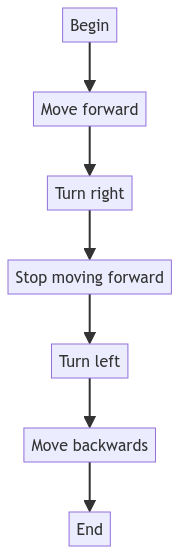
\includegraphics[width=0.2\linewidth]{flowchart_stage1.png}
        \caption{Stage 1 flowchart}
    \end{figure}
    \textbf{Stage 2:}
    \begin{figure}[H]
        \centering
        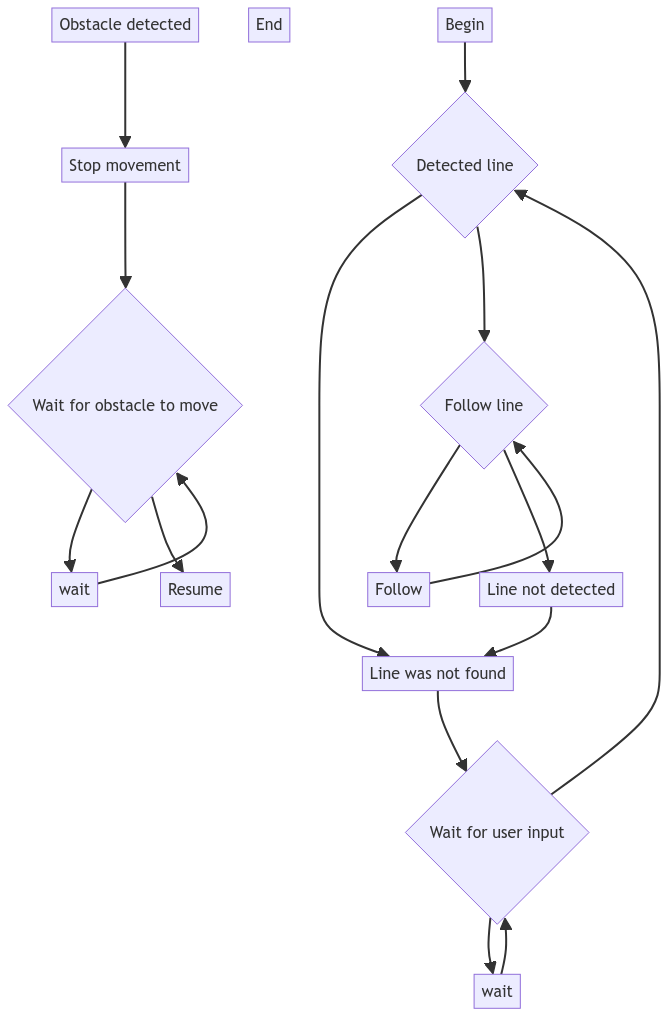
\includegraphics[width=0.5\linewidth]{flowchart_stage2.png}
        \caption{Stage 2 flowchart}
    \end{figure}

    \subsubsection{Version control}
    Effective planning of the Git branch structure is crucial for software
    development projects. When employing Git as a collaboration tool, it is
    imperative to ensure that the team adheres to specific guidelines:
    \begin{itemize}
        \item \textbf{Protected Master Branch:} Only merge requests are permitted on the master branch.
        \item \textbf{Developer Branch Commits:} Commits should be made on the developer branch.
        \item \textbf{Independent Feature Development:} Create a new branch for independent features, branching from the developer branch.
        \item \textbf{Meaningful Commit Messages:} Commit messages should be both meaningful and concise.
        \item \textbf{Peer Review for Merge Requests:} All merge requests must undergo review by another team member.
    \end{itemize}
    These guidelines significantly contribute to the smooth running of the
    development process. Primarily, they prevent the occurrence of large and
    time-consuming merge requests. When followed correctly, these guidelines
    result in a branch structure resembling the illustration in Figure
    \ref{fig:git}.
    \begin{figure}[H]
        \centering
        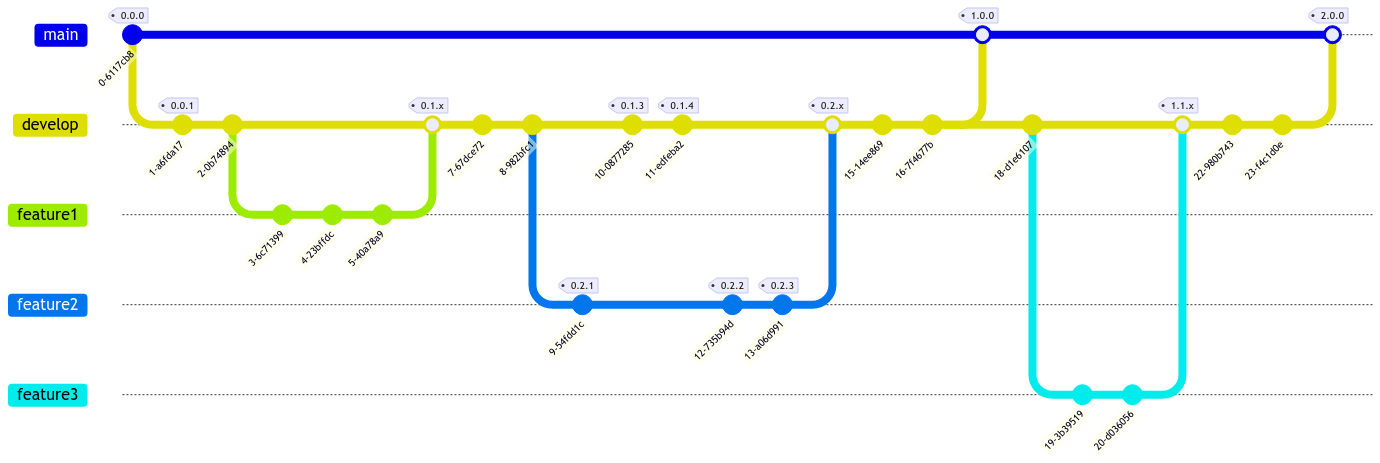
\includegraphics[width=\linewidth]{git.png}
        \caption{Git branch structure}
        \label{fig:git}
    \end{figure}
\end{document}